\section{Simulation of user behavior}
On past semester the IT security group of the chair "Internet Technologies and Systems" worked on the project "Machine Learning for Security Analytics powered by SAP HANA". Within this project the group aimed to implement and test the machine learning approach for security analytics based on SAP HANA. Under this approach the group focused on the analysis of user events, particularly login and logout events. For testing of machine learning analytics module, we have generated several simple brute-force attacks. Also there was the idea to try the machine learning approach powered on SAP HANA for security analytics with more sophisticated cases. But the main problem of trying the approach with sophisticated cases is the lack of data. As we mentioned in the introduction section, mostly only industrial companies have such data in needed amount but they do not share them because of security and privacy. For example, login and logout events contain information about users and this information can not be passed to third parties. We were faced with the task to implement a tool to simulate particular user scenarios, user behavior and as result generate necessary data for further analysis. This simulation tool must provide capability to simulate normal and abnormal scenarios to be able to analyze user behavior by the machine learning approach to detect anomalies.  
  
% with Windows Active Directory
\subsection{Environment description}
We started with designing and describing the test network. Our test network contains the domain controller (DC) node with installed Widows Sever 2012, wiki and database servers Windows Server 2003 and four client computers with Windows 7 Professional 64-bit. To complete the installation, we created four user accounts. All the above information is presented below in the form of compact lists.

\begin{compactitem}
\item [\textbf{Description of the network:}]
\item 4 client computers with Windows 7 Professional 64-bit.
\item Domain controller with Widows Server 2012.
\item Wiki server with Windows Server 2003.
\item Database server with Windows Server 2003.
\end{compactitem}

\begin{compactitem}
\item [\textbf{Users:}]
\item Ivanov
\item Petrov
\item Smirnov
\item Admin
\end{compactitem}
     
\subsection{Normal scenario}
In our configuration, all users have access to client computers, the wiki server and the database server, but only admin has direct access to the domain controller. In the case of the normal scenario, users log into client computers by their credentials and they do it several times per day. Users Petrov and Smirnov during the workday visit the wiki server, but Ivanov does not visit the wiki server despite that he has access. All users have access to the database server, but no one uses it in the normal scenario. In turn, admin usually logs into to his computer and during the workday he logs into to the domain controller, the database server and the wiki server by the remote desktop connection (RDP). The description of the normal behavior you can see on the Figure 1. The lines show all allowed access to computers. The solid lines illustrate access which are used by users, the dash lines show access which are not used by users in the normal behavior despite that they have access. 

\begin{figure}[ht!]
\centering
%[width=90mm]
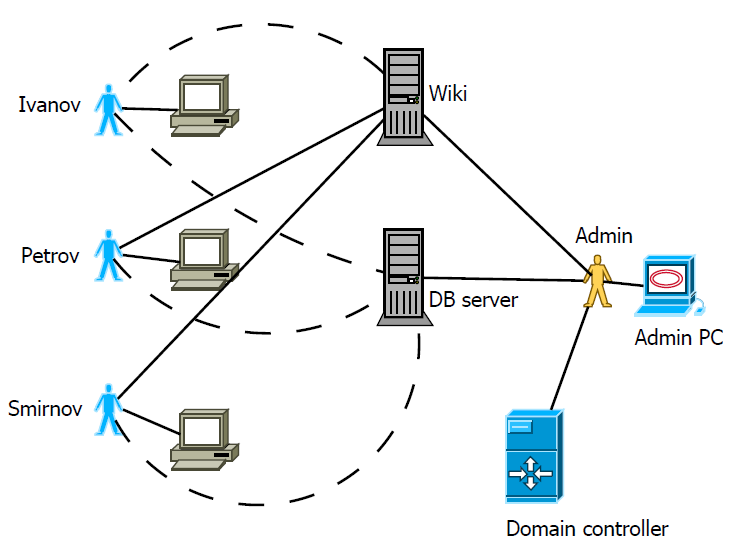
\includegraphics[width=\textwidth]{scenario_normal.png}
\caption{Normal scenario}
\label{overflow}
\end{figure}

\subsection{Abnormal scenario}
The abnormal scenario is the scenario that differs from the normal scenario by some unusual but acceptable behavior. In our case, the abnormal scenario includes additional user behavior. The first abnormal behavior is that the user Ivanov uses the wiki server. This behavior is abnormal but not suspicious, because other users use it every day. The second abnormal behavior is that the user Petrov uses the database server but in the normal scenario no one uses it. This user behavior is more suspicious and could be determined as an attempt to compromise the system. The abnormal scenario is illustrated on the Figure 2. The straight solid lines show normal user behavior, the curve solid line from Ivanov to the wiki server shows the first abnormal behavior and the curve solid line from Petrov to the database server shows the second abnormal behavior that is suspicious and could be determined as an attempt to compromise the system. 
\begin{figure}[ht!]
\centering
%[width=90mm]
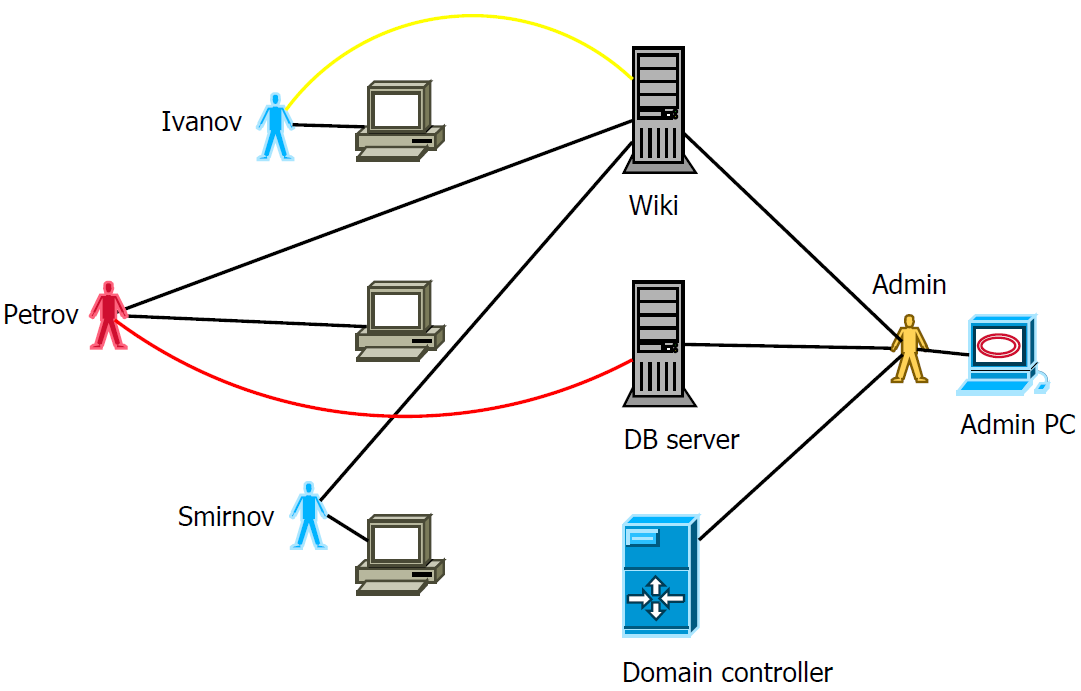
\includegraphics[width=\textwidth]{scenario_abnormal.png}
\caption{Abnormal scenario}
\label{overflow}
\end{figure}

\subsection{Implementation}
The first part of the implementation is the deployment and the configuration of the test environment. To set up the network we used FutureSOC server with installed VMware ESXi. Firstly, we created the network to isolate our virtual machines from others hosted on the same ESXi server. Afterwards, all machines were deployed and configured as described in the section 2.1. We used Windows Server 2012 for the domain controller, Windows Server 2003 for the wiki and database servers and Windows 7 Professional 64-bit for client computers. 

The simulation tool is implemented on the python programming language and uses the virtual network computing protocol (VNC) to connect to virtual machines as the ESXi server supports the VNC protocol. But to use the VNC protocol, firstly, it is needed to enable VNC on the ESXi server, specify the VNC port for each virtual machine and support the VNC protocol on the application side. To use VNC in the simulator, we used the vncdotool library [1]. This library also can take a screenshot of the remote desktop. We used this screenshot functionality for checking a state of the virtual machine by comparing image histograms with predefined states. Once we determined the current state of the virtual machine, we can specify the activities to be undertaken in each case according to the scenario description such as send the ctrl+alt+delete command to the virtual machine, enter the username and the password, open the remote desktop protocol (RDP) connection and others. The RDP connection from the client computer to the database and wiki servers is implemented by invoking the PowerShell script hosted on the virtual machine. This script can accept parameters and it means that we can use the script to establish the connection with any server by specifying the IP address.

In this paragraph, we show how we described the scenario of user behavior. The scenario descriptions are stored in csv files. There are three csv files. The first of them is called computers.csv. It describes all computers that are involved in scenarios and it contains the information about the computer identifier, the IP address or the host, the VNC port, the VNC password and the type of operation system.
The second file is called scenarios.csv. It describes main the user activity that is the connection to the client computer. The file contains the computer identifier referring to the identifier in the computer.csv file, the username, the password, the session time, the count of sessions and the identifier referring to the identifier in the inner-scenarios.csv file. The third file is called inner-scenarios.csv describes the actions of users after logging into the client computer. For example, it can describe the connection to the wiki server, database server or domain controller or even the connection to another client computer. The file contains the identifier, the host, the username, the password and the session time. There are two sets of csv files. The first set is used to perform the normal scenario and the second is used to perform the abnormal scenario, respectively. The described relations between csv files are illustrated on the Figure 3.
 	
\begin{figure}[ht!]
\centering
%[width=90mm]
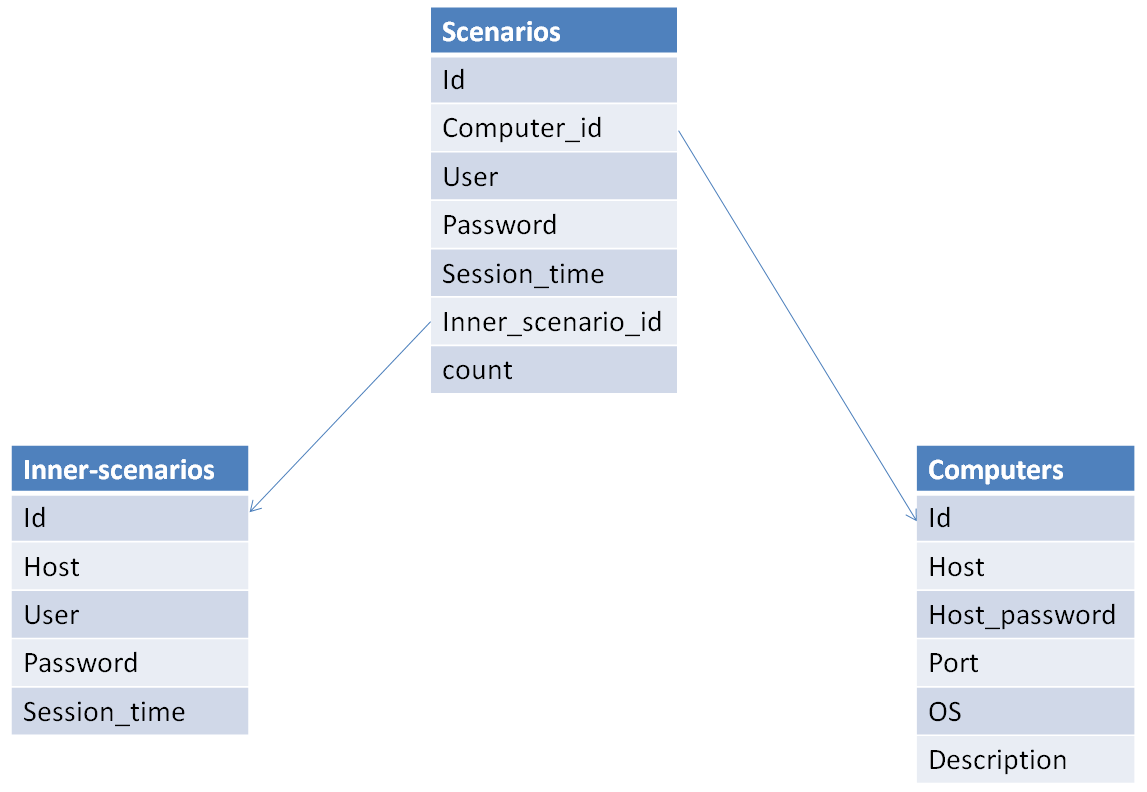
\includegraphics[width=\textwidth]{scenario_relations.png}
\caption{Scenario relations}
\label{overflow}
\end{figure}


%The normal scenario takes about 3,5 hours with 41 login and logout events into client computers and 25 RDP connections to the wiki and database servers. The abnormal scenario takes about 5,5 hours with 45 login and logout events to client computers and 34 RDP connections to the wiki and database servers.
 
%\end{document} 